\documentclass[12pt,a4paper]{article}
\usepackage[utf8]{vietnam}
\usepackage{amsmath,amssymb}
\usepackage{geometry}
\geometry{top=1.2cm,bottom=1.0cm,left=1.3cm,right=1.3cm,headheight=26pt,headsep=10pt,footskip=14pt}
\usepackage{tikz}
\usepackage{xcolor}
\usepackage{enumerate}
\usepackage{graphicx}
\usepackage[version=4]{mhchem}
\usepackage{fancyhdr}
\usepackage{ex_test}

\renewcommand{\baselinestretch}{0.91}
\setlength{\parskip}{0pt}

\definecolor{hfRed}{RGB}{211,47,47}
\definecolor{hfGreen}{RGB}{139,195,144}

\providecommand{\False}{}

\pagestyle{fancy}
\fancyhf{}
\fancyhead[L]{\small\itshape\color{hfRed} Tài liệu lưu hành nội bộ}
\fancyhead[R]{\small\itshape\color{hfRed} Thầy \textbf{TRẦN VĂN THẠNH} - 0777.470.803}
\renewcommand{\headrulewidth}{0.8pt}
\renewcommand{\headrule}{\hbox to\headwidth{\color{hfGreen}\leaders\hrule height \headrulewidth\hfill}}

\fancyfoot[L]{\small\itshape\color{hfRed} CS1: 6/15 Nguyễn Hoàng, P. Kim Long, TP Huế \quad|\quad CS2: 24 Đặng Thái Thân, TP Huế}
\fancyfoot[R]{\small\bfseries\color{hfRed} Trang \thepage}
\renewcommand{\footrulewidth}{0.8pt}
\renewcommand{\footrule}{\hbox to\headwidth{\color{hfGreen}\leaders\hrule height \footrulewidth\hfill}}

\fancypagestyle{firstpage}{
  \fancyhf{}
  \renewcommand{\headrulewidth}{0pt}
  \fancyfoot[L]{\small\itshape\color{hfRed} CS1: 6/15 Nguyễn Hoàng, P. Kim Long, TP Huế \quad|\quad CS2: 24 Đặng Thái Thân, TP Huế}
  \fancyfoot[R]{\small\bfseries\color{hfRed} Trang \thepage}
  \renewcommand{\footrulewidth}{0.8pt}
  \renewcommand{\footrule}{\hbox to\headwidth{\color{hfGreen}\leaders\hrule height \footrulewidth\hfill}}
}

\begin{document}
\thispagestyle{firstpage}

\noindent
\begin{minipage}[t]{0.44\textwidth}
	\centering\fontsize{10pt}{12pt}\selectfont
	\textbf{SỞ GIÁO DỤC VÀ ĐÀO TẠO THỪA THIÊN HUẾ}\\
	\textbf{ĐỀ CHÍNH THỨC}\\
	\textit{(Đề thi có 04 trang)}
\end{minipage}\hfill
\begin{minipage}[t]{0.54\textwidth}
	\centering\small
	\textbf{ĐỀ KIỂM TRA ĐỊNH KỲ CHƯƠNG 2 (CARBOHYDRATE)}\\
	\textbf{MÔN: HOÁ HỌC -- LỚP 12}\\
	\textit{Thời gian làm bài: 50 phút (không kể thời gian phát đề)}\\
	\fbox{\textbf{MÃ ĐỀ: 106}}
\end{minipage}

\smallskip
\begin{center}
	{\color{hfRed}\textbf{\large (BẢN GIÁO VIÊN -- CÓ LỜI GIẢI CHI TIẾT)}}
\end{center}

\smallskip
\noindent\hrulefill
\smallskip

\noindent\textbf{Họ, tên thí sinh:} \dotfill\ \textbf{Lớp:} \dotfill\ \textbf{Số báo danh:} \dotfill

\smallskip
\noindent\textit{(Cho biết nguyên tử khối: H = 1; C = 12; N = 14; O = 16; Na = 23; Mg = 24; S = 32; Cl = 35,5; K = 39; Ca = 40; Fe = 56; Cu = 64; Ag = 108).}

\vspace{0.15cm}
\noindent
\textbf{PHẦN I (4,5 điểm -- 18 câu): Câu trắc nghiệm nhiều phương án lựa chọn.}\\
\textit{Thí sinh trả lời từ câu 1 đến câu 18. Mỗi câu hỏi thí sinh chỉ chọn một phương án.}

\Opensolutionfile{ans}[ans-de06gv]

\begin{ex}
Tinh bột và cellulose đều không thuộc loại
\choice
{\True monosaccharide}
{glucide}
{polysaccharide}
{carbohydrate}
\loigiai{
Tinh bột và cellulose đều thuộc loại polysaccharide (carbohydrate phức tạp tạo bởi nhiều mắt xích glucose), không thuộc loại monosaccharide (đường đơn).\\
\textbf{Chọn A.}}
\end{ex}

\begin{ex}
Trong điều kiện thích hợp glucose lên men tạo thành khí \ce{CO2} và
\choice
{\True \ce{C2H5OH}}
{\ce{CH3COOH}}
{\ce{HCOOH}}
{\ce{CH3CHO}}
\loigiai{
Phương trình lên men rượu: $\ce{C6H12O6 ->[\text{men rượu}][30-35^\circ\text{C}] 2C2H5OH + 2CO2\uparrow}$.\\
\textbf{Chọn A.}}
\end{ex}

\begin{ex}
(SBT -- KNTT). Saccharose thuộc loại carbohydrate nào sau đây?
\choice
{Monosaccharide}
{\True Disaccharide}
{Polysaccharide}
{Oligosaccharide}
\loigiai{
Saccharose có công thức $\ce{C12H22O11}$, được cấu tạo từ một gốc $\alpha$-glucose và một gốc $\beta$-fructose liên kết qua cầu nối oxygen, thuộc loại disaccharide.\\
\textbf{Chọn B.}}
\end{ex}

\begin{ex}
(SBT -- KNTT). Thuỷ phân một phân tử saccharose tạo thành
\choice
{hai phân tử glucose}
{\True một phân tử glucose và một phân tử fructose}
{hai phân tử fructose}
{một phân tử galactose và một phân tử glucose}
\loigiai{
Phương trình thuỷ phân: $\ce{C12H22O11 + H2O ->[H^+,\,t^\circ] C6H12O6 (glucose) + C6H12O6 (fructose)}$.\\
\textbf{Chọn B.}}
\end{ex}

\begin{ex}
(SBT -- KNTT). Phát biểu nào sau đây về cellulose \textbf{không} đúng?
\choice
{Không tan trong nước}
{Là nguồn nguyên liệu sản xuất giấy}
{Có thể phản ứng với \ce{HNO3} tạo cellulose nitrate}
{\True Phản ứng màu với dung dịch iodine}
\loigiai{
Chỉ có tinh bột mới có phản ứng màu xanh tím đặc trưng với dung dịch iodine; cellulose không có cấu trúc xoắn tạo lỗ rỗng hấp phụ iodine nên không có phản ứng này.\\
\textbf{Chọn D.}}
\end{ex}

\begin{ex}
(SBT -- CĐ). Tinh bột và cellulose là các polymer lần lượt tạo bởi các mắt xích
\choice
{$\alpha$-fructose và $\beta$-glucose}
{$\beta$-fructose và $\beta$-glucose}
{\True $\alpha$-glucose và $\beta$-glucose}
{$\alpha$-glucose và $\beta$-fructose}
\loigiai{
Tinh bột gồm các mắt xích $\alpha$-glucose (trong amylose và amylopectin), còn cellulose gồm các mắt xích $\beta$-glucose liên kết với nhau qua liên kết $\beta$-1,4-glycoside.\\
\textbf{Chọn C.}}
\end{ex}

\begin{ex}
(SBT -- CTST). Phát biểu nào sau đây \textbf{không} đúng về glucose và fructose?
\choice
{Chúng đều có công thức phân tử \ce{C6H12O6}}
{Chúng đều là các hợp chất carbohydrate}
{Chúng đều là các monosaccharide}
{\True Chúng có tính chất hoá học tương tự nhau}
\loigiai{
Glucose là polyhydroxy aldehyde, còn fructose là polyhydroxy ketone. Nhóm chức khác nhau dẫn đến tính chất hóa học khác biệt (ví dụ glucose làm mất màu dung dịch nước bromine, còn fructose trong môi trường acid không làm mất màu dung dịch bromine).\\
\textbf{Chọn D.}}
\end{ex}

\begin{ex}
(SBT -- CĐ). Khi đun nóng dung dịch chứa carbohydrate X và \ce{Cu(OH)2} trong môi trường kiềm, X có phản ứng với \ce{Cu(OH)2} tạo kết tủa đỏ gạch. X \textbf{không} thể là
\choice
{\True saccharose}
{glucose}
{fructose}
{maltose}
\loigiai{
Saccharose không có nhóm -OH hemiacetal hay hemiketal tự do (không mở vòng tạo nhóm aldehyde), do đó trong môi trường kiềm không tham gia phản ứng khử \ce{Cu(OH)2} tạo kết tủa đỏ gạch \ce{Cu2O}.\\
\textbf{Chọn A.}}
\end{ex}

\begin{ex}
(SBT -- CĐ). Polymer là nguồn carbohydrate dự trữ có trong cơ thể động vật và được tạo thành từ các đơn vị glucose là
\choice
{cellulose}
{amylose}
{amylopectin}
{\True glycogen}
\loigiai{
Glycogen (tinh bột động vật) là carbohydrate dự trữ năng lượng ở gan và cơ của động vật, được cấu tạo từ các đơn vị $\alpha$-glucose phân nhánh mạnh.\\
\textbf{Chọn D.}}
\end{ex}

\begin{ex}
\begin{minipage}{0.72\textwidth}
Trong công thức cấu tạo dạng mạch vòng $\alpha$-glucose bên cạnh, nhóm -OH hemiacetal là -OH gắn ở nguyên tử carbon số mấy?
\choice
{2}
{3}
{4}
{\True 1}
\end{minipage}\hfill
\begin{minipage}{0.26\textwidth}
\centering
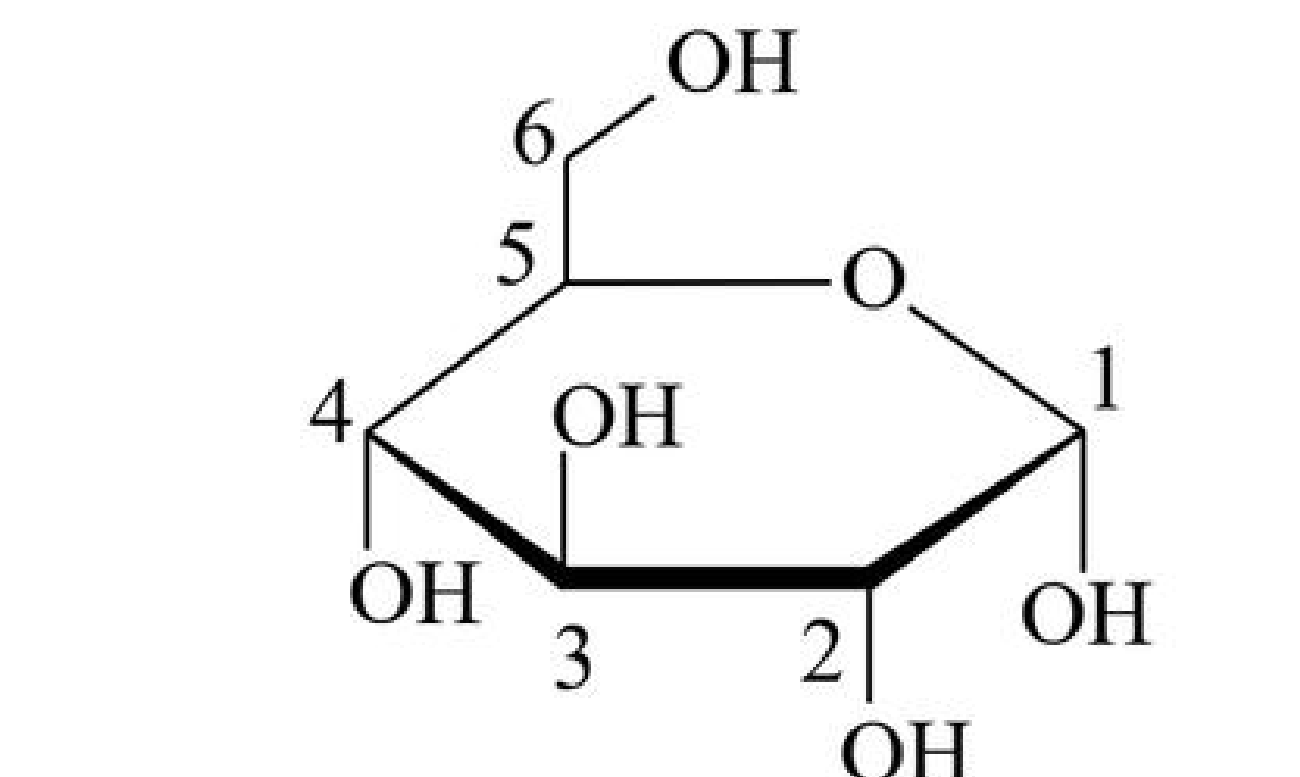
\includegraphics[width=3.5cm]{images_crop_de06/cau10_alpha_glucose.png}
\end{minipage}
\loigiai{
Trong dạng mạch vòng của glucose, nhóm -OH liên kết trực tiếp với nguyên tử carbon C1 (carbon carbonyl khi ở mạch hở) được gọi là nhóm -OH hemiacetal.\\
\textbf{Chọn D.}}
\end{ex}

\begin{ex}
Dung dịch saccharose tinh khiết không có tính khử, nhưng khi đun nóng với dung dịch \ce{H2SO4} lại có thể cho phản ứng tráng gương. Đó là do:
\choice
{Đã có sự tạo thành aldehyde sau phản ứng}
{\True Saccharose bị thuỷ phân tạo thành glucose và fructose}
{Saccharose bị thuỷ phân tạo thành glucose}
{Saccharose bị thuỷ phân tạo thành fructose}
\loigiai{
Khi đun nóng với dung dịch acid \ce{H2SO4} loãng làm xúc tác, saccharose bị thuỷ phân thành hỗn hợp glucose và fructose. Cả hai monosaccharide này đều có phản ứng tráng gương.\\
\textbf{Chọn B.}}
\end{ex}

\begin{ex}
Phát biểu nào sau đây \textbf{sai}?
\choice
{\True Thủy phân saccharose chỉ thu được glucose}
{Glucose có khả năng tham gia phản ứng tráng bạc}
{Cellulose và tinh bột đều thuộc loại polysaccharide}
{Cellulose có cấu tạo mạch không phân nhánh}
\loigiai{
Thủy phân saccharose thu được cả glucose và fructose, do đó phát biểu A sai.\\
\textbf{Chọn A.}}
\end{ex}

\begin{ex}
(SBT -- CTST). Mạch nha là tên gọi khác của carbohydrate nào sau đây?
\choice
{Glucose}
{Fructose}
{Saccharose}
{\True Maltose}
\loigiai{
Maltose còn có tên gọi dân gian là đường mạch nha (malt sugar), có nhiều trong mầm lúa mạch.\\
\textbf{Chọn D.}}
\end{ex}

\begin{ex}
Polysaccharide X là chất rắn, màu trắng, dạng sợi. Trong bông nõn có gần 98\% chất X. Thủy phân X, thu được monosaccharide Y. Phát biểu nào sau đây đúng?
\choice
{\True Y có tính chất của alcohol đa chức}
{X có phản ứng tráng bạc}
{Phân tử khối của Y bằng 342}
{X dễ tan trong nước}
\loigiai{
Chất X là cellulose, thủy phân X thu được glucose (Y). Glucose là polyhydroxy aldehyde nên mang tính chất của alcohol đa chức (hòa tan \ce{Cu(OH)2} ở nhiệt độ thường tạo phức màu xanh lam).\\
\textbf{Chọn A.}}
\end{ex}

\begin{ex}
(SBT -- CTST). Chất nào sau đây \textbf{không} phải polymer sinh học?
\choice
{Tinh bột}
{Cellulose}
{\True Glucosamine}
{Chitin}
\loigiai{
Glucosamine là monosaccharide dẫn xuất amin (phân tử đơn lẻ), không phải là polymer sinh học. Tinh bột, cellulose và chitin đều là polymer thiên nhiên.\\
\textbf{Chọn C.}}
\end{ex}

\begin{ex}
Cho các phát biểu sau về ứng dụng và trạng thái tự nhiên của glucose và fructose:\\
(a) Cả glucose và fructose đều là chất rắn, dễ tan trong nước, có vị ngọt.\\
(b) Glucose có nhiều trong quả chín (nhất là nho chín), fructose có nhiều trong mật ong.\\
(c) Dung dịch truyền tĩnh mạch là glucose 5\%.\\
(d) Glucose và fructose chủ yếu đóng vai trò cung cấp năng lượng cho tế bào.\\
Số phát biểu đúng là:
\choice
{3}
{\True 4}
{1}
{2}
\loigiai{
Cả 4 phát biểu (a), (b), (c), (d) đều đúng.\\
\textbf{Chọn B.}}
\end{ex}

\begin{ex}
Cho các phát biểu sau:\\
(a) Glucose được gọi là đường nho do có nhiều trong quả nho chín.\\
(b) Chất béo là diester của glycerol với acid béo.\\
(c) Phân tử amylopectin có cấu trúc mạch phân nhánh.\\
(d) Ở nhiệt độ thường, triolein ở trạng thái rắn.\\
(e) Trong mật ong chứa nhiều fructose.\\
(f) Tinh bột là một trong những lương thực cơ bản của con người.\\
Số phát biểu đúng là:
\choice
{5}
{6}
{3}
{\True 4}
\loigiai{
- (a) Đúng.\\
- (b) Sai, chất béo là triester của glycerol với acid béo.\\
- (c) Đúng, amylopectin có nhánh nhờ liên kết $\alpha$-1,6-glycoside.\\
- (d) Sai, triolein là chất béo không no nên ở trạng thái lỏng ở nhiệt độ thường.\\
- (e) Đúng, fructose chiếm khoảng 40\% trong mật ong.\\
- (f) Đúng, tinh bột là lương thực chính.\\
=> Có 4 phát biểu đúng là (a), (c), (e), (f).\\
\textbf{Chọn D.}}
\end{ex}

\begin{ex}
(SBT -- CTST). Cho các phát biểu sau về carbohydrate:\\
(a) Saccharose và fructose không phải là đường khử.\\
(b) Amylopectin phân nhánh là do sự xuất hiện của liên kết $\alpha$-1,6-glycoside.\\
(c) Cellulose không phân nhánh do chỉ xuất hiện liên kết $\beta$-1,4-glycoside.\\
(d) Số nhóm -OH trong phân tử saccharose là 8.\\
Số phát biểu đúng là:
\choice
{1}
{2}
{\True 3}
{4}
\loigiai{
- (a) Sai, fructose là đường khử vì trong môi trường kiềm có cân bằng chuyển hoá thành glucose.\\
- (b) Đúng, liên kết $\alpha$-1,6-glycoside tạo nhánh.\\
- (c) Đúng, liên kết $\beta$-1,4-glycoside tạo chuỗi mạch thẳng.\\
- (d) Đúng, phân tử saccharose có 8 nhóm -OH (\ce{C12H14O3(OH)8}).\\
=> Có 3 phát biểu đúng là (b), (c), (d).\\
\textbf{Chọn C.}}
\end{ex}

\Closesolutionfile{ans}



\vspace{0.15cm}
\noindent
\textbf{PHẦN II (4,0 điểm -- 4 câu): Câu trắc nghiệm đúng sai.}\\
\textit{Thí sinh trả lời từ câu 1 đến câu 4. Trong mỗi ý a), b), c), d) ở mỗi câu, thí sinh chọn đúng hoặc sai.}

\setcounter{ex}{0}

\begin{ex}
(SBT -- KNTT).
\choiceTF
{\True Glucose và fructose đều có công thức phân tử là \ce{C6H12O6}}
{\True Glucose và fructose đều tồn tại dạng mạch hở và mạch vòng}
{\False Glucose và fructose đều là pentahydroxy aldehyde}
{\False Dạng vòng của glucose và fructose đều là vòng sáu cạnh}
\loigiai{
a) Đúng, cả 2 đều có CTPT là \ce{C6H12O6}.\\
b) Đúng, trong dung dịch luôn có sự chuyển hóa qua lại giữa dạng mạch hở và mạch vòng.\\
c) Sai, glucose là pentahydroxy aldehyde, còn fructose là pentahydroxy ketone.\\
d) Sai, dạng vòng của glucose chủ yếu là vòng 6 cạnh, còn fructose chủ yếu là vòng 5 cạnh.\\
\textbf{Đáp án: a - Đ, b - Đ, c - S, d - S.}}
\end{ex}

\begin{ex}
Cấu trúc phân tử saccharose như sau:
{\centering
	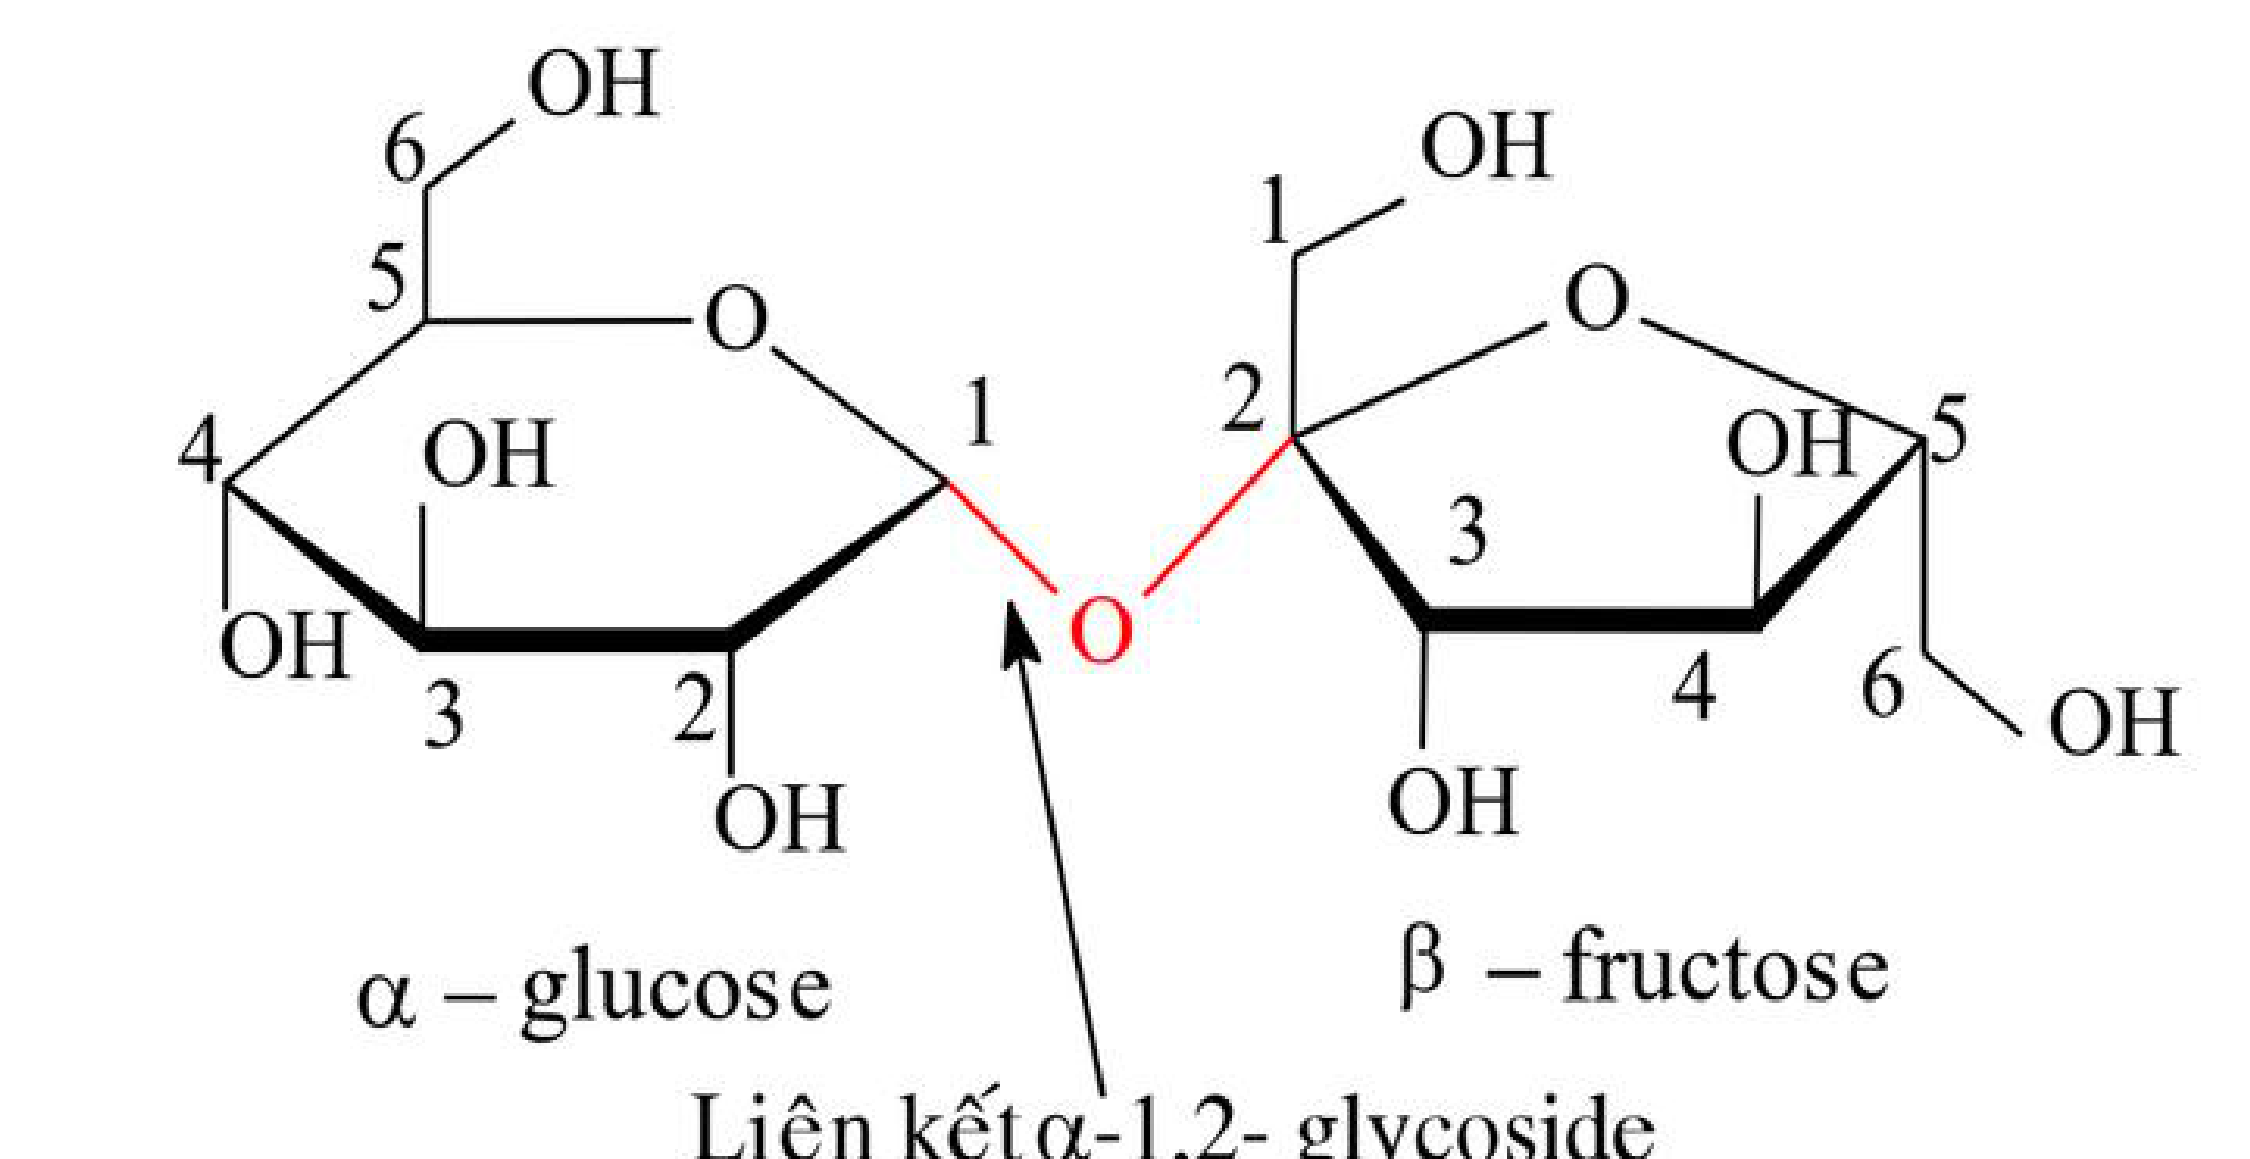
\includegraphics[width=3.6cm]{images_crop_de06/p2_cau2_saccharose.png}\par}
\choiceTF
{\True Phân tử saccharose gồm một gốc $\alpha$-glucose và một gốc $\beta$-fructose}
{\False Phân tử saccharose có chứa nhóm -OH hemiacetal}
{\False Phân tử saccharose có chứa nhóm -OH hemiketal}
{\True Hai gốc monosaccharide trong saccharose được liên kết với nhau bởi một nguyên tử oxygen}
\loigiai{
a) Đúng, saccharose tạo bởi một gốc $\alpha$-glucose và một gốc $\beta$-fructose.\\
b) Sai, nhóm -OH hemiacetal ở C1 của glucose đã tham gia liên kết glycoside.\\
c) Sai, nhóm -OH hemiketal ở C2 của fructose đã tham gia liên kết glycoside.\\
d) Đúng, hai gốc monosaccharide nối với nhau qua cầu nguyên tử oxygen (liên kết $\alpha$-1,2-glycoside).\\
\textbf{Đáp án: a - Đ, b - S, c - S, d - Đ.}}
\end{ex}

\begin{ex}
Tiến hành thí nghiệm phản ứng của hồ tinh bột với iodine theo các bước sau đây:\\
\textit{Bước 1:} Cho vài giọt dung dịch iodine vào ống nghiệm đựng sẵn 2 mL dung dịch hồ tinh bột.\\
\textit{Bước 2:} Đun nóng dung dịch một lát, sau đó để nguội.
{\centering
	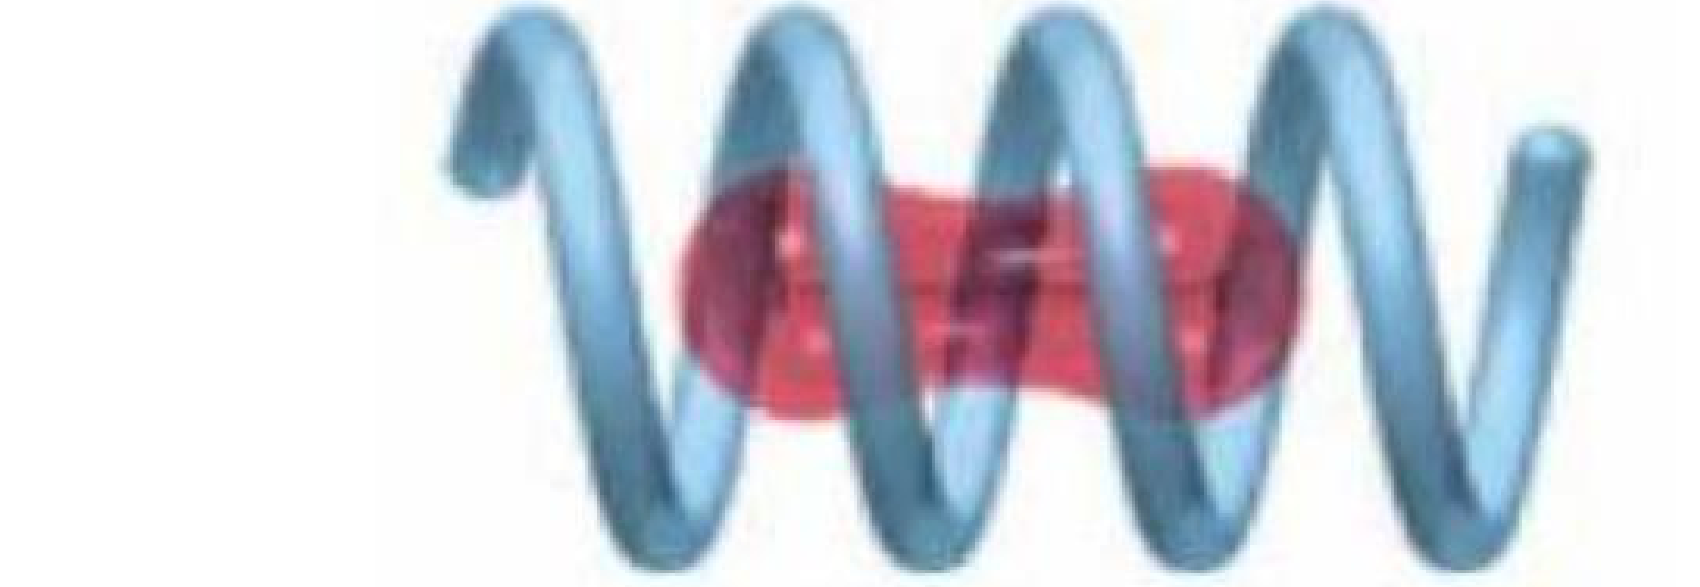
\includegraphics[width=2.5cm]{images_crop_de06/p2_cau3_tinh_bot_iodine.png}\\
	{\footnotesize\itshape\color{hfRed}\textbf{Mô hình tương tác giữa tinh bột \& iodine}}\par}
\choiceTF
{\False Sau bước 1, dung dịch thu được có màu xanh tím. Sau bước 2, dung dịch bị mất màu}
{\True Mạch tinh bột xoắn lại tạo các lỗ rỗng, các lỗ rỗng này hấp phụ \ce{I2} tạo nên hợp chất màu xanh tím}
{\False Nếu nhỏ vài giọt dung dịch iodine lên mặt cắt của quả chuối chín thì màu xanh tím cũng xuất hiện}
{\True Có thể dùng dung dịch iodine để phân biệt hai dung dịch riêng biệt gồm hồ tinh bột và saccharose}
\loigiai{
a) Sai, sau bước 2 (khi đã để nguội), màu xanh tím xuất hiện trở lại (mất màu khi đun nóng).\\
b) Đúng, cấu trúc xoắn của amylose giữ các phân tử \ce{I2} trong lỗ rỗng tạo phức màu xanh tím.\\
c) Sai, chuối chín tinh bột đã chuyển hóa thành glucose và fructose nên không cho màu xanh tím.\\
d) Đúng, hồ tinh bột hóa xanh tím, saccharose không hiện tượng.\\
\textbf{Đáp án: a - S, b - Đ, c - S, d - Đ.}}
\end{ex}

\begin{ex}
Thí nghiệm phản ứng của cellulose với nitric acid:\\
\textbf{Hoá chất:} cellulose (bông), dung dịch \ce{HNO3} đặc, dung dịch \ce{H2SO4} đặc, dung dịch \ce{NaHCO3} loãng, quỳ tím.\\
\textbf{Dụng cụ:} cốc thuỷ tinh 100 mL, chậu nước nóng, chậu nước đá, đũa thuỷ tinh, giấy lọc, đĩa sứ, đèn cồn.\\
\textbf{Tiến hành:}\\
\textit{Bước 1:} Cho khoảng 5 mL dung dịch \ce{HNO3} đặc vào cốc thuỷ tinh ngâm trong chậu nước đá. Thêm từ từ khoảng 10 mL dung dịch \ce{H2SO4} đặc vào cốc và khuấy đều.\\
\textit{Bước 2:} Lấy cốc ra khỏi chậu nước đá, thêm tiếp một nhúm bông vào cốc và dùng đũa thuỷ tinh ấn bông ngập trong dung dịch. Ngâm cốc trong chậu nước nóng khoảng 10 phút.\\
\textit{Bước 3:} Để nguội, lấy sản phẩm ra khỏi cốc, rửa nhiều lần với nước lạnh (đến khi nước rửa không đổi màu quỳ tím), sau đó rửa lại bằng dung dịch \ce{NaHCO3} loãng. Ép sản phẩm giữa hai miếng giấy lọc và làm khô tự nhiên. Sau đó, để sản phẩm lên đĩa sứ rồi đốt cháy.
{\centering
	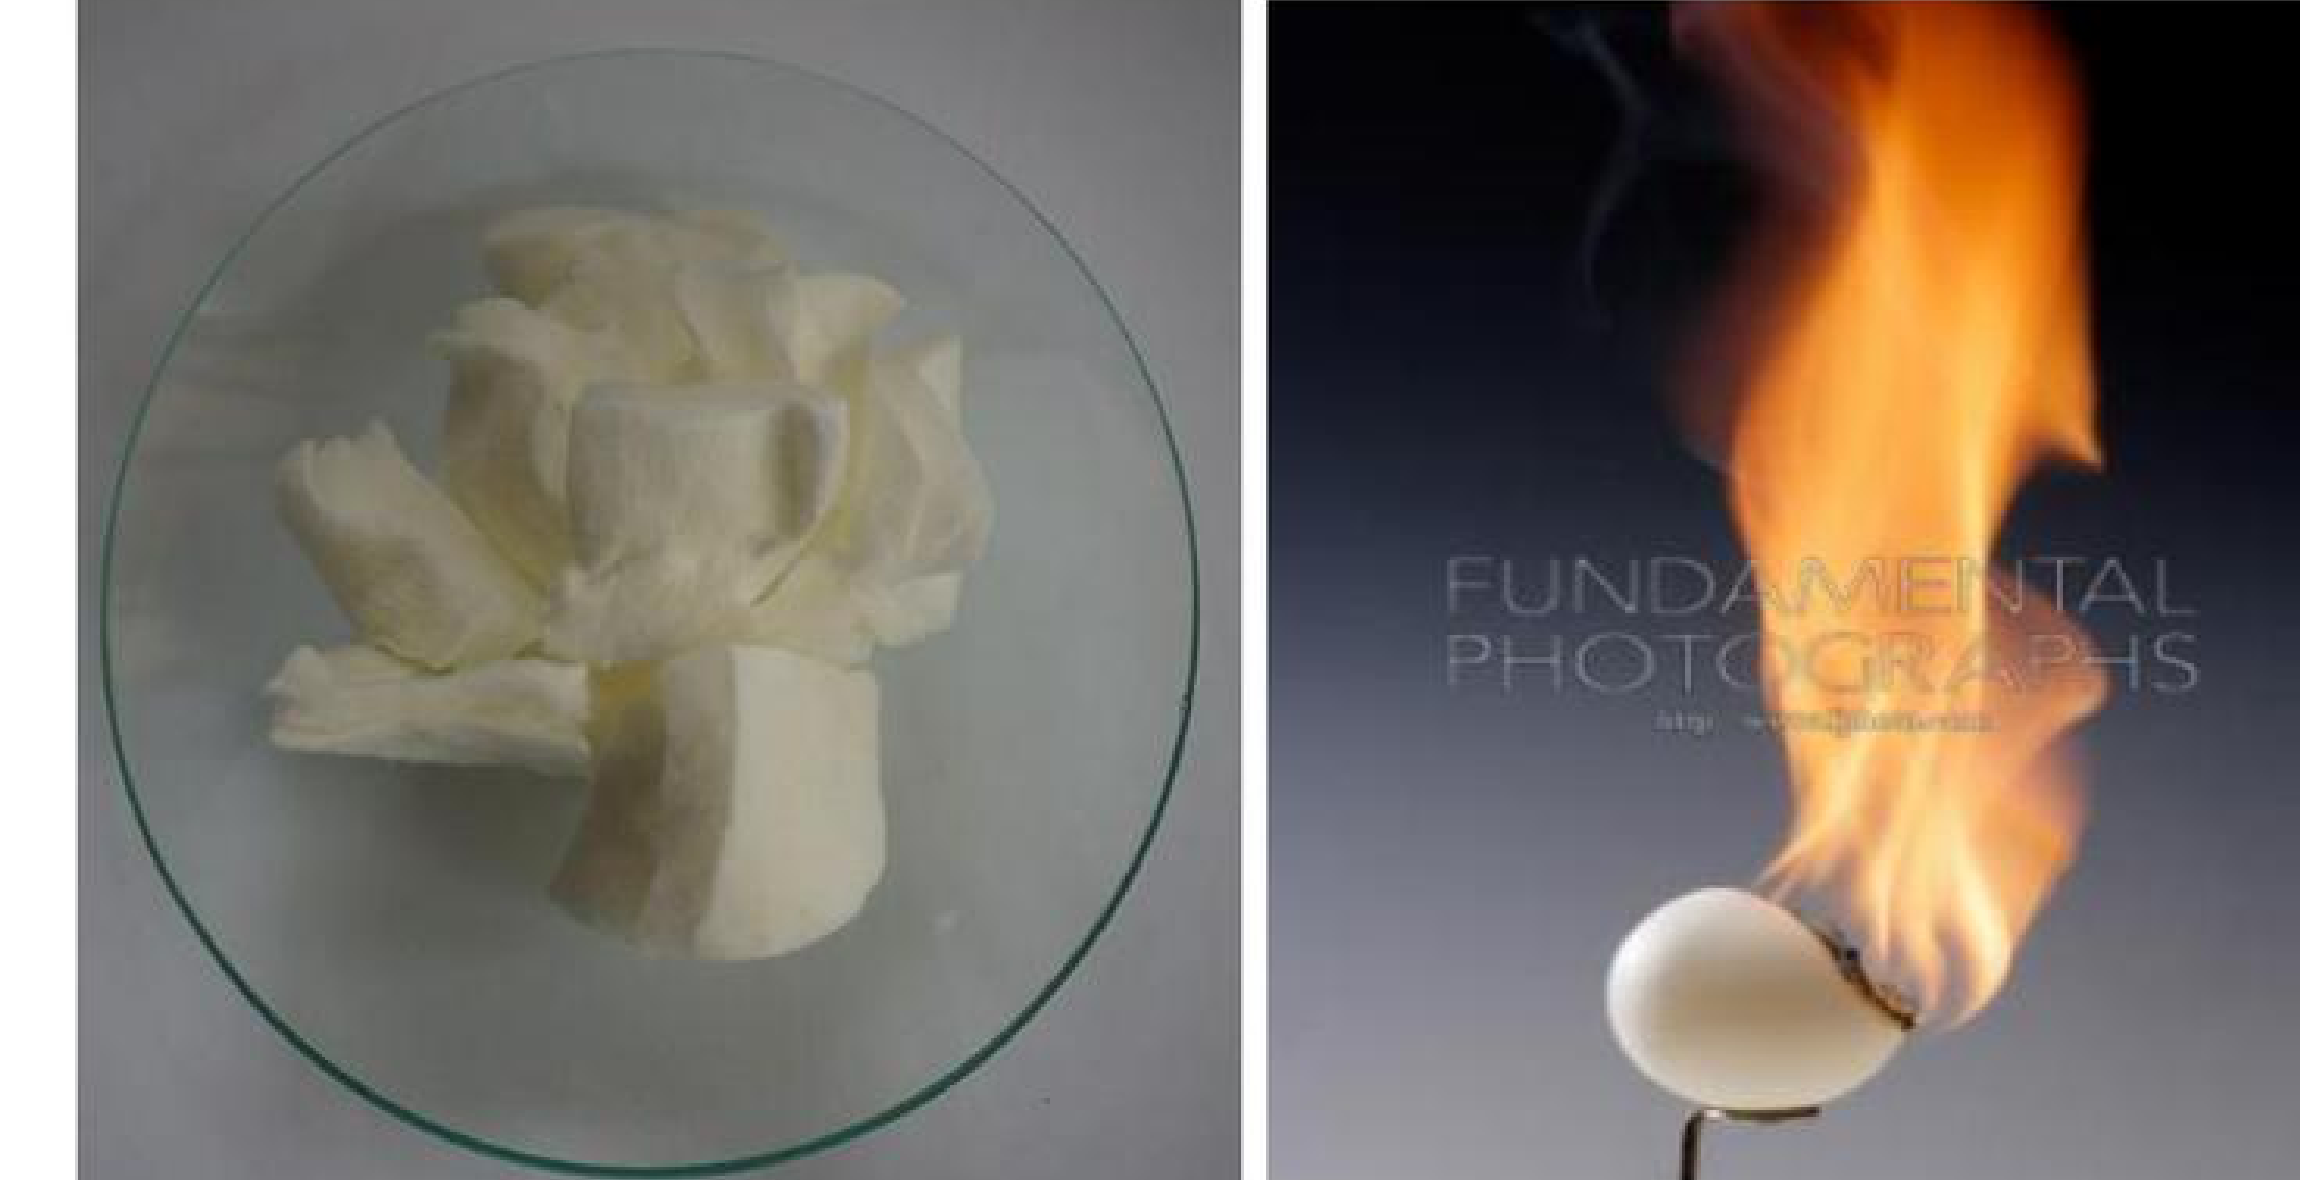
\includegraphics[width=3.6cm]{images_crop_de06/p2_cau4_cellulose_trinitrate.png}\\
	{\footnotesize\itshape\color{hfRed}\textbf{Cellulose trinitrate \qquad\qquad Cellulose trinitrate cháy}}\par}
\choiceTF
{\True Sau bước 3, sản phẩm thu được có màu vàng}
{\False Có thể thay thế nhúm bông bằng tinh bột}
{\False Sau bước 3, lấy sản phẩm thu được đốt cháy thấy có khói trắng xuất hiện}
{\True Thí nghiệm trên chứng minh mỗi mắt xích trong phân tử cellulose có 3 nhóm OH tự do}
\loigiai{
a) Đúng, cellulose trinitrate thu được có màu vàng ngà.\\
b) Sai, tinh bột bị acid đặc phân hủy mạnh tạo khối nhầy keo dính, không tạo sợi thuốc súng.\\
c) Sai, cellulose trinitrate là thuốc súng không khói, khi cháy bùng cháy rất nhanh không sinh khói.\\
d) Đúng, phản ứng thế este hoá tạo $[\ce{C6H7O2(ONO2)3}]_n$ chứng minh mỗi mắt xích có 3 nhóm -OH tự do.\\
\textbf{Đáp án: a - Đ, b - S, c - S, d - Đ.}}
\end{ex}



\vspace{0.15cm}
\noindent
\textbf{PHẦN III (1,5 điểm -- 6 câu): Câu trắc nghiệm yêu cầu trả lời ngắn.}\\
\textit{Thí sinh trả lời từ câu 1 đến câu 6. Mỗi câu hỏi thí sinh điền câu trả lời vào ô tương ứng.}

\setcounter{ex}{0}

\begin{ex}
Cho các chất: saccharose, glucose, fructose, formic acid và acetic aldehyde. Trong các chất trên, số chất vừa có khả năng tham gia phản ứng tráng bạc vừa có khả năng phản ứng với \ce{Cu(OH)2} ở điều kiện thường là bao nhiêu?
\loigiai{
- Tác dụng với \ce{Cu(OH)2} ở đk thường: glucose, fructose, saccharose (polyalcohol có $\ge 2$ nhóm -OH kề nhau) và formic acid (acid carboxylic).\\
- Tráng bạc: glucose, fructose, formic acid, acetic aldehyde.\\
=> Vừa tráng bạc vừa tác dụng với \ce{Cu(OH)2} ở đk thường gồm 3 chất: glucose, fructose, formic acid.\\
\textbf{Đáp số: 3.}}
\noindent\textbf{Đáp số: \color{hfRed}{3}}
\end{ex}

\begin{ex}
\begin{minipage}{0.65\textwidth}
Phân tử maltose ở dạng mạch vòng (hình bên) có bao nhiêu nhóm alcohol bậc 2?
\loigiai{
Quan sát công thức mạch vòng của maltose:\\
- Gốc $\alpha$-glucose thứ nhất (vòng bên trái): các nhóm -OH ở C2, C3, C4 gắn với C bậc 2 $\to$ có 3 nhóm alcohol bậc 2.\\
- Gốc $\alpha$-glucose thứ hai (vòng bên phải): các nhóm -OH ở C2, C3 gắn với C bậc 2 $\to$ có 2 nhóm alcohol bậc 2 (nhóm -OH ở C1 là hemiacetal; nhóm ở C6 là bậc 1).\\
=> Tổng số nhóm alcohol bậc 2 là $3 + 2 = \mathbf{5}$.\\
\textbf{Đáp số: 5.}}
\noindent\textbf{Đáp số: \color{hfRed}{5}}
\end{minipage}\hfill
\begin{minipage}{0.33\textwidth}
\centering
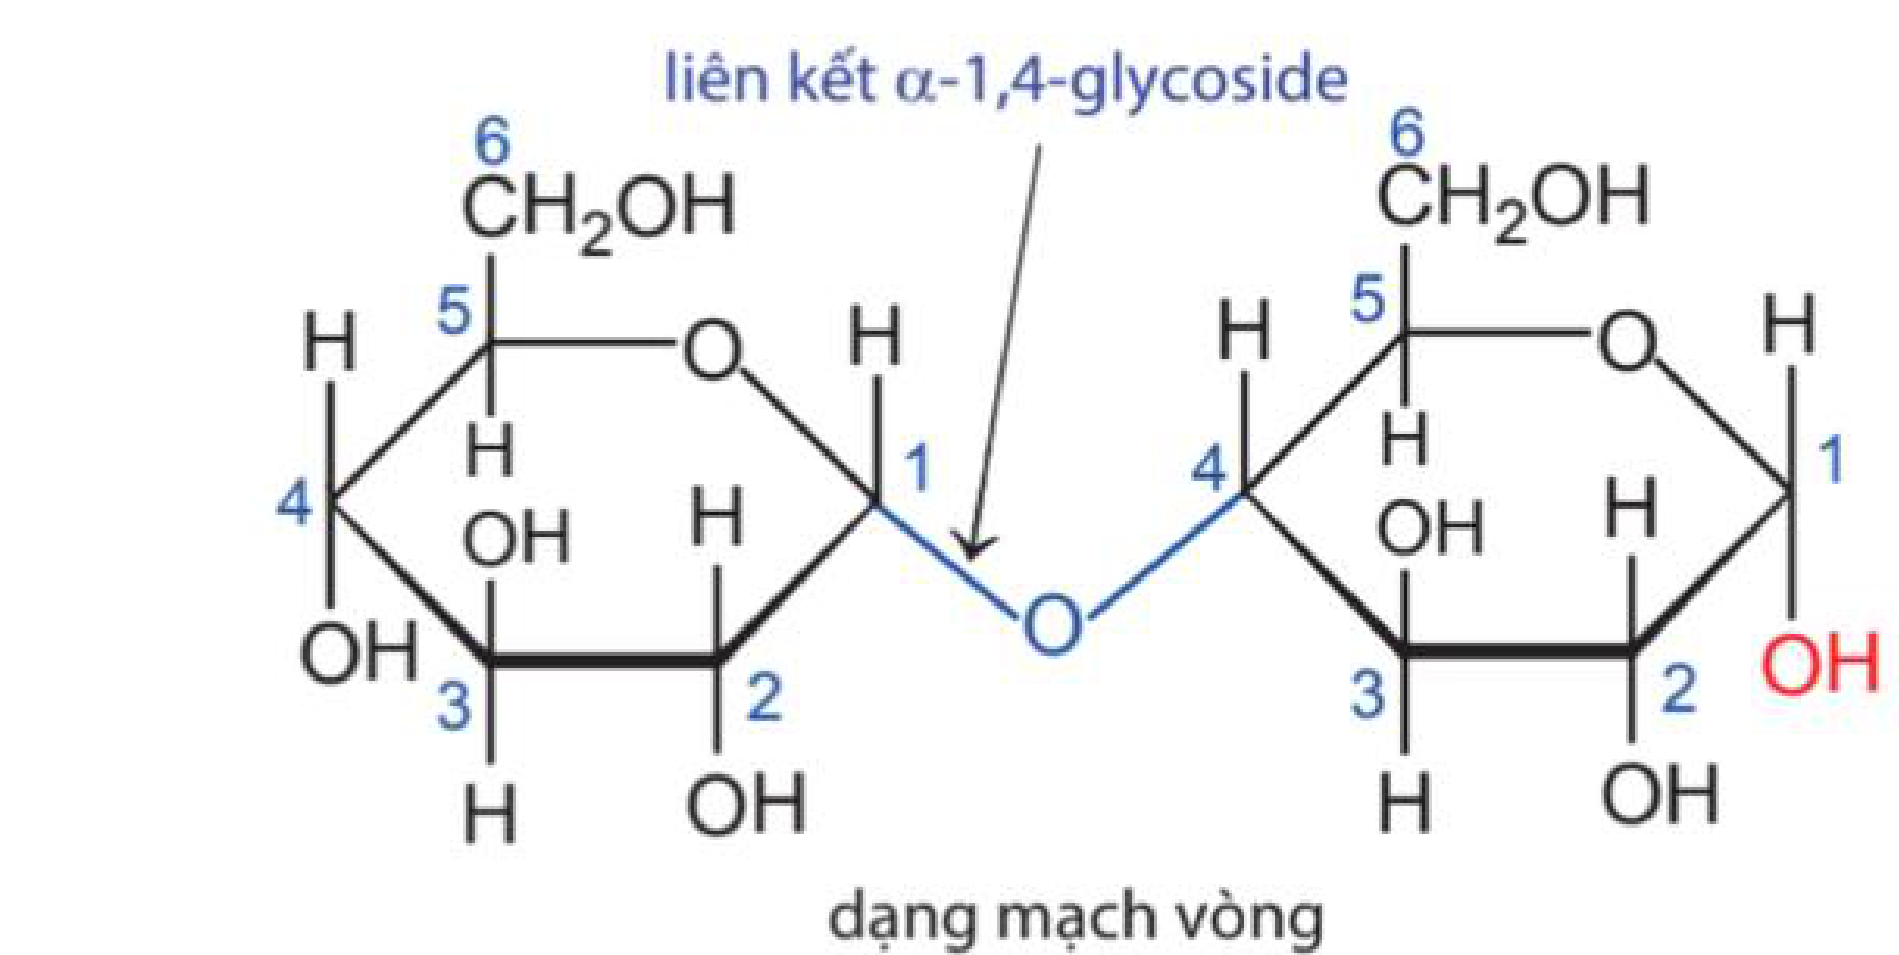
\includegraphics[width=4.8cm]{images_crop_de06/p3_cau2_maltose.png}
\end{minipage}
\end{ex}

\begin{ex}
Cho các phản ứng sau: hoà tan \ce{Cu(OH)2} ở nhiệt độ thường tạo dung dịch xanh lam, phản ứng với thuốc thử Tollens, \ce{Cu(OH)2}/\ce{OH^-} ($t^\circ$), thủy phân môi trường acid, phản ứng màu với dung dịch iodine, phản ứng với \ce{HNO3} đặc/\ce{H2SO4} đặc ($t^\circ$). Số phản ứng mà cellulose có khả năng tham gia phản ứng là
\loigiai{
Cellulose chỉ tham gia 2 phản ứng trong danh sách trên:\\
1. Thủy phân trong môi trường acid tạo glucose.\\
2. Phản ứng với \ce{HNO3} đặc / \ce{H2SO4} đặc ($t^\circ$) tạo cellulose trinitrate.\\
\textbf{Đáp số: 2.}}
\noindent\textbf{Đáp số: \color{hfRed}{2}}
\end{ex}

\begin{ex}
Trong y học, glucose làm thuốc tăng lực cho người bệnh, dễ hấp thu và cung cấp khá nhiều năng lượng. Phản ứng oxi hóa glucose tạo thành \ce{CO2} và \ce{H2O} cung cấp năng lượng cho cơ thể. Một người bệnh được truyền hai chai chứa 250 mL dung dịch glucose 5\%. Tính năng lượng tối đa bệnh nhân nhận được từ các chai truyền glucose đó. Biết nhiệt tạo thành của glucose \ce{C6H12O6}, \ce{CO2} và \ce{H2O} lần lượt là $-1\,271\text{ kJ/mol}$, $-393{,}5\text{ kJ/mol}$ và $-285{,}8\text{ kJ/mol}$; dung dịch glucose 5\% có khối lượng riêng là $1{,}019\text{ g/mL}$. (Làm tròn kết quả đến hàng đơn vị).
\loigiai{
- Phản ứng nhiệt hoá học: $\ce{C6H12O6 + 6O2 -> 6CO2 + 6H2O}$.\\
  $\Delta_r H^\circ_{298} = 6 \cdot (-393{,}5) + 6 \cdot (-285{,}8) - (-1271) = -2804{,}8\text{ kJ}$.\\
  Do đó khi oxi hóa 1 mol glucose tỏa ra $2804{,}8\text{ kJ}$.\\
- Khối lượng dung dịch 2 chai: $m_{\text{dd}} = 2 \times 250 \times 1{,}019 = 509{,}5\text{ g}$.\\
- Khối lượng glucose: $m_{\text{glucose}} = 509{,}5 \times 5\% = 25{,}475\text{ g}$.\\
- Năng lượng bệnh nhân nhận được: $Q = \dfrac{25{,}475}{180} \times 2804{,}8 \approx \mathbf{397\text{ kJ}}$.\\
\textbf{Đáp số: 397.}}
\noindent\textbf{Đáp số: \color{hfRed}{397}}
\end{ex}

\begin{ex}
Trong công nghiệp, saccharose là nguyên liệu để thủy phân thành glucose và fructose dùng trong kĩ thuật tráng gương, ruột phích. Để thu được 30 kg glucose cần thuỷ phân $m\text{ kg}$ saccharose với hiệu suất phản ứng là 60\%. Giá trị của $m$ là
\loigiai{
- Phương trình thủy phân: $\ce{C12H22O11 + H2O -> C6H12O6 (glucose) + C6H12O6 (fructose)}$.\\
  Theo lí thuyết: $342\text{ kg}$ saccharose tạo ra $180\text{ kg}$ glucose.\\
- Khối lượng saccharose cần theo lí thuyết: $m_{\text{LT}} = 30 \times \dfrac{342}{180} = 57\text{ kg}$.\\
- Vì hiệu suất $H = 60\%$ nên thực tế cần: $m = 57 \times \dfrac{100}{60} = \mathbf{95\text{ kg}}$.\\
\textbf{Đáp số: 95.}}
\noindent\textbf{Đáp số: \color{hfRed}{95}}
\end{ex}

\begin{ex}
Một người nông dân có 5 sào ruộng để cấy lúa (3 sào lấy thóc dùng làm thức ăn và 2 sào dùng nấu rượu (ethyl alcohol). Biết năng suất của mỗi sào lúa là $180\text{ kg/sào}$ và một năm thu hoạch 2 vụ. Hàm lượng tinh bột trong gạo là 70\%, biết $1\text{ kg}$ thóc sau khi xát sẽ thu được $0{,}7\text{ kg}$ gạo, ethyl alcohol được nấu là $30^\circ$ với hiệu suất đạt 75\% (khối lượng riêng của ethyl alcohol $D = 0{,}8\text{ g/mL}$). Nếu được bán với giá $20.000\text{ đồng/lít}$ thì số tiền thu được từ việc bán rượu (ethyl alcohol) trong một năm của người nông dân là $a\text{ triệu đồng}$ (làm tròn một chữ số thập phân). Tính $a$.
\loigiai{
- Khối lượng thóc dùng nấu rượu trong 1 năm (2 sào, 2 vụ):\\
  $m_{\text{thóc}} = 2 \times 180 \times 2 = 720\text{ kg}$.\\
- Khối lượng gạo thu được: $m_{\text{gạo}} = 720 \times 0{,}7 = 504\text{ kg}$.\\
- Khối lượng tinh bột thực tế phản ứng (hiệu suất $75\%$):\\
  $m_{\text{tinh bột}} = 504 \times 70\% \times 75\% = 264{,}6\text{ kg}$.\\
- Số mol mắt xích tinh bột: $n = \dfrac{264{,}6}{162} = \dfrac{49}{30}\text{ kmol}$.\\
- Số mol ethanol thu được: $n_{\text{ethanol}} = 2 \times \dfrac{49}{30} = \dfrac{49}{15}\text{ kmol}$.\\
- Khối lượng ethanol: $m_{\text{ethanol}} = \dfrac{49}{15} \times 46 = \dfrac{2254}{15}\text{ kg}$.\\
- Thể tích ethanol nguyên chất: $V_{\text{ethanol}} = \dfrac{2254}{15} : 0{,}8 = \dfrac{1127}{6}\text{ lít}$.\\
- Thể tích rượu $30^\circ$ thu được: $V_{\text{rượu}} = \dfrac{1127}{6} : 0{,}3 \approx 626{,}11\text{ lít}$.\\
- Số tiền thu được:\\
  $\text{Tiền} = 626{,}11 \times 20.000 = 12.522.222\text{ đồng} \approx \mathbf{12{,}5\text{ triệu đồng}}$.\\
\textbf{Đáp số: 12,5.}}
\noindent\textbf{Đáp số: \color{hfRed}{12,5}}
\end{ex}


\newpage
\noindent
{\color{hfRed}\textbf{\Large BẢNG ĐÁP ÁN ĐỀ KIỂM TRA SỐ 6 (CHƯƠNG 2: CARBOHYDRATE)}}

\vspace{0.3cm}
\noindent\textbf{PHẦN I:}
\begin{center}
\input{ans-de06gv}
\end{center}

\vspace{0.2cm}
\noindent\textbf{PHẦN II:}
\begin{center}
\begin{tabular}{|c|c|c|c|c|}
\hline
\textbf{Câu} & \textbf{Ý a} & \textbf{Ý b} & \textbf{Ý c} & \textbf{Ý d} \\ \hline
\textbf{1} & Đ & Đ & S & S \\ \hline
\textbf{2} & Đ & S & S & Đ \\ \hline
\textbf{3} & S & Đ & S & Đ \\ \hline
\textbf{4} & Đ & S & S & Đ \\ \hline
\end{tabular}
\end{center}

\vspace{0.2cm}
\noindent\textbf{PHẦN III:}
\begin{center}
\begin{tabular}{|c|c|c|c|c|c|}
\hline
\textbf{Câu 1} & \textbf{Câu 2} & \textbf{Câu 3} & \textbf{Câu 4} & \textbf{Câu 5} & \textbf{Câu 6} \\ \hline
3 & 5 & 2 & 397 & 95 & 12,5 \\ \hline
\end{tabular}
\end{center}

\par\vspace{0.1cm}
\centerline{\textbf{---------- HẾT ----------}}

\end{document}
